\documentclass[a4paper, 12pt]{article}
% packages
\usepackage{amssymb}
\usepackage[fleqn]{mathtools}
\usepackage{tikz}
\usepackage{enumerate}
\usepackage{bussproofs}
\usepackage{xcolor}
\usepackage[margin=1.3cm]{geometry}
\usepackage{logicproof}
\usepackage{diagbox}
\usepackage{listings}
\usepackage{graphicx}
\usepackage{lstautogobble}
\usepackage{hyperref}
\usepackage{multirow}
\usepackage{tipa}
\usetikzlibrary{decorations.pathreplacing, arrows, shapes.gates.logic.US, circuits.logic.US, calc, automata, positioning}

% shorthand for verbatim
% this clashes with logicproof, so maybe fix this at some point?
\catcode`~=\active
\def~#1~{\texttt{#1}}

% code listing
\lstdefinestyle{main}{
    numberstyle=\tiny,
    breaklines=true,
    showspaces=false,
    showstringspaces=false,
    tabsize=2,
    numbers=left,
    basicstyle=\ttfamily,
    columns=fixed,
    fontadjust=true,
    basewidth=0.5em,
    autogobble,
    xleftmargin=3.0ex,
    mathescape=true
}
\newcommand{\dollar}{\mbox{\textdollar}} %
\lstset{style=main}

% augmented matrix
\makeatletter
\renewcommand*\env@matrix[1][*\c@MaxMatrixCols c]{%
\hskip -\arraycolsep
\let\@ifnextchar\new@ifnextchar
\array{#1}}
\makeatother

% ceiling / floor
\DeclarePairedDelimiter{\ceil}{\lceil}{\rceil}
\DeclarePairedDelimiter{\floor}{\lfloor}{\rfloor}

% custom commands
\newcommand{\indefint}[2]{\int #1 \, \mathrm{d}#2}
\newcommand{\defint}[4]{\int_{#1}^{#2} #3 \, \mathrm{d}#4}
\newcommand{\pdif}[2]{\frac{\partial #1}{\partial #2}}
\newcommand{\dif}[2]{\frac{\mathrm{d}#1}{\mathrm{d}#2}}
\newcommand{\limit}[2]{\raisebox{0.5ex}{\scalebox{0.8}{$\displaystyle{\lim_{#1 \to #2}}$}}}
\newcommand{\summation}[2]{\sum\limits_{#1}^{#2}}
\newcommand{\intbracket}[3]{\left[#3\right]_{#1}^{#2}}
\newcommand{\ulsmash}[1]{\underline{\smash{#1}}}

\newcommand{\powerset}[0]{\wp}
\renewcommand{\emptyset}[0]{\varnothing}

\makeatletter
\newsavebox{\@brx}
\newcommand{\llangle}[1][]{\savebox{\@brx}{\(\m@th{#1\langle}\)}%
  \mathopen{\copy\@brx\kern-0.5\wd\@brx\usebox{\@brx}}}
\newcommand{\rrangle}[1][]{\savebox{\@brx}{\(\m@th{#1\rangle}\)}%
  \mathclose{\copy\@brx\kern-0.5\wd\@brx\usebox{\@brx}}}
\makeatother
\newcommand{\lla}{\llangle}
\newcommand{\rra}{\rrangle}
\newcommand{\la}{\langle}
\newcommand{\ra}{\rangle}

\newcommand{\mat}[1]{\boldsymbol{#1}}
\renewcommand{\vec}[1]{\boldsymbol{#1}}
\newcommand{\rowt}[1]{\begin{bmatrix}
    #1
\end{bmatrix}^\top}

\newcommand{\unaryproof}[2]{\AxiomC{#1} \UnaryInfC{#2} \DisplayProof}
\newcommand{\binaryproof}[3]{\AxiomC{#1} \AxiomC{#2} \BinaryInfC{#3} \DisplayProof}
\newcommand{\trinaryproof}[4]{\AxiomC{#1} \AxiomC{#2} \AxiomC{#3} \TrinaryInfC{#4} \DisplayProof}

\newcommand{\axiom}[1]{\AxiomC{#1}}
\newcommand{\unary}[1]{\UnaryInfC{#1}}
\newcommand{\binary}[1]{\BinaryInfC{#1}}
\newcommand{\trinary}[1]{\TrinaryInfC{#1}}
\newcommand{\quaternary}[1]{\QuaternaryInfC{#1}}
\newcommand{\quinary}[1]{\QuinaryInfC{#1}}
\newcommand{\dproof}[0]{\DisplayProof}

\newcommand{\bnfsep}[0]{\ |\ }
\newcommand{\concsep}[0]{\ ||\ }
\newcommand{\violet}[1]{\textcolor{violet}{#1}}
\newcommand{\blue}[1]{\textcolor{blue}{#1}}
\newcommand{\red}[1]{\textcolor{red}{#1}}

% no indent
\setlength\parindent{0pt}

% reasoning proofs
\usepackage{ltablex}
\usepackage{environ}
\keepXColumns
\NewEnviron{reasoning}{
    \begin{tabularx}{\textwidth}{rlX}
        \BODY
    \end{tabularx}
}
\newcommand{\proofline}[3]{$(#1)$ & $#2$ & \hfill #3 \smallskip \\}
\newcommand{\proofarbitrary}[1]{& take arbitrary $#1$ \smallskip \\}
\newcommand{\prooftext}[1]{\multicolumn{3}{l}{#1} \smallskip \\}
\newcommand{\proofmath}[3]{$#1$ & = $#2$ & \hfill #3 \smallskip \\}
\newcommand{\prooftherefore}[1]{& $\therefore #1$ \smallskip \\}
\newcommand{\proofbc}[0]{\prooftext{\textbf{Base Case}}}
\newcommand{\proofis}[0]{\prooftext{\textbf{Inductive Step}}}

% reasoning er diagrams
\newcommand{\nattribute}[4]{
    \node[draw, state, inner sep=0cm, minimum size=0.2cm, label=#3:{#4}] (#1) at (#2) {};
}
\newcommand{\mattribute}[4]{
    \node[draw, state, accepting, inner sep=0cm, minimum size=0.2cm, label=#3:{#4}] (#1) at (#2) {};
}
\newcommand{\dattribute}[4]{
    \node[draw, state, dashed, inner sep=0cm, minimum size=0.2cm, label=#3:{#4}] (#1) at (#2) {};
}
\newcommand{\entity}[3]{
    \node[] (#1-c) at (#2) {#3};
    \node[inner sep=0cm] (#1-l) at ($(#1-c) + (-1, 0)$) {};
    \node[inner sep=0cm] (#1-r) at ($(#1-c) + (1, 0)$) {};
    \node[inner sep=0cm] (#1-u) at ($(#1-c) + (0, 0.5)$) {};
    \node[inner sep=0cm] (#1-d) at ($(#1-c) + (0, -0.5)$) {};
    \draw
    ($(#1-c) + (-1, 0.5)$) -- ($(#1-c) + (1, 0.5)$) -- ($(#1-c) + (1, -0.5)$) -- ($(#1-c) + (-1, -0.5)$) -- cycle;
}
\newcommand{\relationship}[3]{
    \node[] (#1-c) at (#2) {#3};
    \node[inner sep=0cm] (#1-l) at ($(#1-c) + (-1, 0)$) {};
    \node[inner sep=0cm] (#1-r) at ($(#1-c) + (1, 0)$) {};
    \node[inner sep=0cm] (#1-u) at ($(#1-c) + (0, 1)$) {};
    \node[inner sep=0cm] (#1-d) at ($(#1-c) + (0, -1)$) {};
    \draw
    ($(#1-c) + (-1, 0)$) -- ($(#1-c) + (0, 1)$) -- ($(#1-c) + (1, 0)$) -- ($(#1-c) + (0, -1)$) -- cycle;
}

% actual document
\begin{document}
    \section*{CO233 - Computational Techniques}
        \subsection*{15th January 2020}
            \subsubsection*{Vector and Matrix Norms}
                An orthonormal basis of $\mathbb{R}^n$ are unit vectors that are pairwise mutually perpendicular; such that for $(e_1, \cdots, e_n)$;
                \begin{itemize}
                    \itemsep0em
                    \item $e_i \cdot e_i = 1$
                    \item $e_i \cdot e_j = 0$, if $i \neq j$
                \end{itemize}
                The standard canonical basis of $\mathbb{R}^3$ are the $i,j,k$ vectors, and similar in $\mathbb{R}^2$.
                However, we can form another orthonormal basis of $\mathbb{R}^2$ by bisecting the angles as such;
                \begin{center}
                    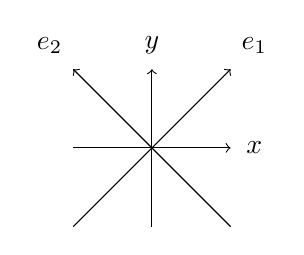
\begin{tikzpicture}
                        \node (y) at (0, 1.3) {$y$};
                        \node (x) at (1.3, 0) {$x$};
                        \node (e1) at (1.3, 1.3) {$e_1$};
                        \node (e2) at (-1.3, 1.3) {$e_2$};
                        \draw
                        (0, -1) edge[->] (0, 1)
                        (-1, 0) edge[->] (1, 0)
                        (-1, -1) edge[->] (1, 1)
                        (1, -1) edge[->] (-1, 1);
                    \end{tikzpicture}
                \end{center}
                If we take a vector $\vec{v} \in \mathbb{R}^n$, the Euclidean norm (or the $\ell_2$-norm) is defined as such;
                \begin{center}
                    $|| \vec{v} ||_2 = \sqrt{\summation{i=1}{n} v_i^2}$
                \end{center}
                A norm, a mapping $||\ || : \mathbb{R}^n \to \mathbb{R}^+$, must satisfy these 3 axioms;
                \begin{enumerate}[(i)]
                    \itemsep0em
                    \item $|| \vec{v} || > 0$ given that $\vec{v} \neq \vec{0}$
                    \item $|| \lambda \vec{v} || = |\lambda|\ || \vec{v} ||$
                    \item $|| \vec{v} + \vec{w} || \leq || \vec{v} || + || \vec{w} ||$ (triangular inequality)
                \end{enumerate}
                Some other ($\ell_p$) norms are defined as follows;
                \begin{align*}
                    \ell_1\text{-norm } || \vec{v} ||_1 & = \summation{i=1}{n}|v_i| \\
                    \ell_\infty\text{-norm } || \vec{v} ||_\infty & = \max \{|v_i| : 1 \leq i \leq n\} \\
                    \ell_p\text{-norm } || \vec{v} ||_p & = \left(\summation{i=1}{n} |v_i|^p\right)^\frac{1}{p}
                \end{align*}
                In each dimension, we have the following;
                \begin{itemize}
                    \itemsep0em
                    \item $n = 1$
                        \begin{itemize}
                            \itemsep0em
                            \item $|| \vec{v} ||_1 = | v | = | v |$
                            \item $|| \vec{v} ||_2 = \sqrt{v^2} = | v |$
                            \item $|| \vec{v} ||_\infty = \max \{| v |\} = | v |$
                        \end{itemize}
                    \item $n = 2$
                        \smallskip

                        We can represent this geometrically as such;
                        \begin{center}
                            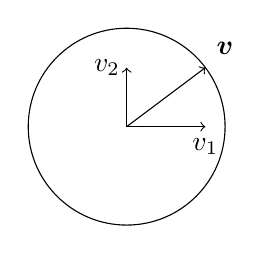
\begin{tikzpicture}[x=0.25cm, y=0.25cm]
                                \node at (4, -1) {$v_1$};
                                \node at (-1, 3) {$v_2$};
                                \node at (5, 4) {$\vec{v}$};

                                \draw (0, 0) circle (5);
                                \draw (0, 0) edge[->] (4, 0);
                                \draw (0, 0) edge[->] (0, 3);
                                \draw (0, 0) edge[->] (4, 3);
                            \end{tikzpicture}
                        \end{center}
                        In our case $|| \vec{v} ||_\infty = \max\{ | v_1 |, | v_2 | \} = | v_1 |$, but the point is that it's either of the "sides" of the triangle.
                        Obviously, $|| \vec{v} ||_2 \geq || \vec{v} ||_\infty$, as it's the hypotenuse of the triangle, and similarly, $|| \vec{v} ||_1 \geq || \vec{v} ||_2$, due to the triangle inequality.
                        Therefore we have $|| \vec{v} ||_1 \geq || \vec{v} ||_2 \geq || \vec{v} ||_\infty$.
                        \smallskip

                        Even if the orthonormal base changes, the Euclidean norm stays the same, whereas the other norms can change.
                        As such, we can say the $\ell_2$-norm is invariant under an \textbf{orthogonal transformation} (a basis change from an orthonormal bases to another orthonormal bases).
                    \item $n =\ ?$ (general)
                        \smallskip

                        The goal is to prove $|| \vec{v} ||_\infty \leq || \vec{v} ||_2 \leq || \vec{v} ||_1$.
                        If we first take the squares of all of them, such that we have the following;
                        \begin{align*}
                            || \vec{v} ||_1^2 & = \left(\summation{i = 1}{n} | v_i |\right)^2 \\
                            || \vec{v} ||_2^2 & = \summation{i = 1}{n} | v_i |^2 \\
                            || \vec{v} ||_\infty^2 & = (\max\{| v_i | : 1 \leq i \leq n\})^2 \\
                        \end{align*}
                        Since the $\ell_\infty$-norm corresponds to a single $v_i$, it's obvious that the following inequality holds (since the $\ell_2$-norm squared has all the other terms squared, as well as the $\ell_\infty$-norm squared);
                        \begin{center}
                            $|| \vec{v} ||_2^2 = \summation{i = 1}{n} | v_i |^2 \geq (\max\{| v_i | : 1 \leq i \leq n\})^2 = || \vec{v} ||_\infty^2 \Rightarrow || \vec{v} ||_2 \geq || \vec{v} ||_\infty$
                        \end{center}
                        To prove the other inequality, we see that the square of the sum of absolutes is greater than the sum of the squares, as the square of the sum contains the cross terms (which will be positive).
                        \begin{center}
                            $|| \vec{v} ||_2^2 = \summation{i = 1}{n} | v_i |^2 \leq \left(\summation{i = 1}{n} | v_i |\right)^2 = || \vec{v} ||_\infty^1 \Rightarrow || \vec{v} ||_2 \leq || \vec{v} ||_1$
                        \end{center}
                        As such, we can conclude that $|| \vec{v} ||_\infty \leq || \vec{v} ||_2 \leq || \vec{v} ||_1$ in any dimension. \hfill $\blacksquare$
                \end{itemize}
            \subsubsection*{Tutorial Question}
                Find the locus of vectors such that $|| \vec{v} ||_p \leq 1$, for $p = \red{1}, \blue{2}, \violet{\infty}$ in $n = 2$;
                \begin{center}
                    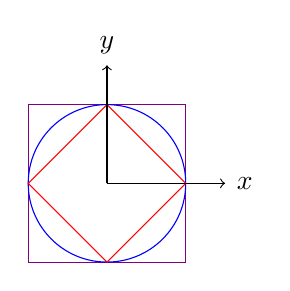
\begin{tikzpicture}
                        \node at (1.75, 0) {$x$};
                        \node at (0, 1.75) {$y$};

                        \draw[violet] (-1, 1) -- (1, 1) -- (1, -1) -- (-1, -1) -- cycle;
                        \draw[blue] (0, 0) circle (1);
                        \draw[red] (0, 1) -- (1, 0) -- (0, -1) -- (-1, 0) -- cycle;
                        \draw
                        (0, 0) edge[->] (1.5, 0)
                        (0, 0) edge[->] (0, 1.5);
                    \end{tikzpicture}
                \end{center}
                Imagine they're all shaded from the border to the origin.
            \subsubsection*{$\ell_p$-norm}
                Our goal is to show that as $p \to \infty$, we get the definition of the $\ell_\infty$-norm previously stated.
                Take a vector $\vec{v} \in \mathbb{R}^n$, where both $\vec{v}$ and $n$ are fixed.
                \begin{center}
                    $|| \vec{v} ||_p^p = \summation{i = 1}{n} | v_i |^p$
                \end{center}
                Obviously, this is greater than or equal to $|| \vec{v} ||_\infty^p$, as it would only be a single $| v_i |^p$.
                Similarly, it must be less than or equal to $n | v_i |^p$, as $v_i$ is the maximum of all the components.
                \begin{center}
                    $|| \vec{v} ||_\infty^p \leq || \vec{v} ||_p^p = \summation{i = 1}{n} | v_i |^p \leq n || \vec{v} ||_\infty^p$
                \end{center}
                Taking everything to the power of $\frac{1}{p}$, we obtain the following result (note that $p > 0$ hence the signs don't change);
                \begin{center}
                    $|| \vec{v} ||_\infty \leq || \vec{v} ||_p = \leq n^\frac{1}{p} || \vec{v} ||_\infty$
                \end{center}
                As $p \to \infty$, since $n \geq 2$ ($n = 1$ is shown to collapse to the same component), we have $n^\frac{1}{p} \to 1$, which sandwiches the middle term.
            \subsubsection*{Some Proposition ($\ell_\infty$-norm vs $\ell_2$-norm)}
                The proposition is as follows; for a vector $\vec{v} \in \mathbb{R}^n$, $|| \vec{v} ||_2 \leq \sqrt{n} || \vec{v} ||_\infty$.
                To show this, we know that each of $| v_i |$ is less than or equal to $|| \vec{v} ||_\infty$, by definition of the maximum.
                The same can be said for $| v_i |^2$, vs $|| \vec{v} ||_\infty^2$.
                Taking square roots, we have the following;
                \begin{center}
                    $|| \vec{v} ||_2^2 = \summation{i = 1}{n} | v_i |^2 \leq n || \vec{v} ||_\infty^2 \Rightarrow || \vec{v} ||_2 \leq \sqrt{n} || \vec{v} ||_\infty$
                \end{center}
                To show this holds similarly for $|| \vec{v} ||_1 \leq \sqrt{n} || \vec{v} ||_2$, we employ the Cauchy-Schwarz inequality, which states $| \vec{x} \cdot \vec{y} | \leq || \vec{x} ||_2 || \vec{y} ||_2$.
                The Cauchy-Schwarz inequality uses the fact that $\vec{x} \cdot \vec{y} = || \vec{x} ||_2 || \vec{y} ||_2 \cos \theta$.
                To do this, we need to define a sign function $\text{sgn} : \mathbb{R} \to \{1, -1\}$ as follows;
                \begin{align*}
                    \text{sgn}\ x & = \begin{cases}
                        1 & x \geq 0 \\
                        -1 & x < 0
                    \end{cases}
                    \intertext{We also need to craft a vector $\vec{w}$, as follows;}
                    w_i & = \frac{\text{sgn}\ v_i}{\sqrt{n}} & 1 \leq i \leq n \\
                    \vec{v} \cdot \vec{w} & = \summation{i = 1}{n} v_i w_i \\
                    & = \summation{i = 1}{n} \frac{v_i \cdot \text{sgn}\ v_i}{\sqrt{n}} & \text{product of same sign becomes positive} \\
                    & = \summation{i = 1}{n} \frac{| v_i |}{\sqrt{n}} \\
                    & = \sqrt{n} \summation{i = 1}{n} | v_i | \\
                    & = \sqrt{n} || \vec{v} ||_1 \\
                    || \vec{w} ||_2 & = \summation{i = 1}{n} \frac{\pm 1}{\sqrt{n}}^2 \\
                    & = \summation{i = 1}{n} \frac{1}{n} \\
                    & = 1
                \end{align*}
                By \violet{Cauchy-Schwarz}, we get;
                \begin{center}
                    $\sqrt{n} || \vec{v} ||_1 = \violet{| \vec{v} \cdot \vec{w} | \leq || \vec{v} ||_2 || \vec{w} ||_2} = || \vec{v} ||_2$
                \end{center}
        \subsection*{16th January 2020}
            Note that this recording has \textbf{no audio}, and therefore will just be the board transcribed.
            I honestly have no idea what he was doing in this lecture, it seems to just jump from topic to topic.
            \subsubsection*{Equivalence of Norms?}
                Take any two norms on $\mathbb{R}^n$; $||\ ||_a$, and $||\ ||_b$.
                \begin{center}
                    $\exists r, s \in \mathbb{R}^+\ \forall \vec{v} \in \mathbb{R}^n\ [r || \vec{v} ||_b \leq || \vec{v} ||_a \leq s || \vec{v} ||_b]$
                \end{center}
                This means that norms in finite dimensional vector spaces are equivalent (no idea why, look it up).
            \subsubsection*{Convergence of Vector Sequences}
                $(\vec{r}_n)$ is a sequence of vectors, and $(a_{i, j})$ is the $i, j^\text{th}$ entry of $\mat{A}$.
                For a vector $\vec{v}^{(m)} \in \mathbb{R}^n$, where $m = 0, 1, 2, \dots$
                \begin{align*}
                    \vec{v}^{(m)} & = \begin{bmatrix}
                        v_1^{(m)} \\ v_2^{(m)} \\ \vdots \\ v_n^{(m)}
                    \end{bmatrix}
                \end{align*}
                For a vector sequence $\vec{v}^{(m)}$ to converge to some vector $\vec{v} \in \mathbb{R}^n$, the following must hold;
                \begin{center}
                    $\vec{v}^{(m)} \to \vec{v} \in \mathbb{R}^n \Leftrightarrow \limit{m}{\infty} || \vec{v}^{(m)} - \vec{v} || \to 0$
                \end{center}
                This is componentwise convergence, such that $\forall i \in [1, n]\ [v_i^{(m)} \to v_i]$.
            \subsubsection*{Matrix Norms}
                Vectors are a type of matrix.
                For a matrix $\mat{A} \in \mathbb{R}^{m \times n}$, the following properties of its norms must hold, where $||\ || : \mathbb{R}^{m \times n} \to \mathbb{R}_{\geq 0}$;
                \begin{enumerate}[(i)]
                    \itemsep0em
                    \item $|| \mat{A} || > 0$ given that $\mat{A} \neq \mat{0}$
                    \item $|| \lambda \mat{A} || = | \lambda | || \mat{A} ||$
                    \item $|| \mat{A} + \mat{B} || \leq || \mat{A} || + || \mat{B} ||$
                    \item $|| \mat{B} \mat{A} || \leq || \mat{B} || || \mat{A} ||$
                \end{enumerate}
                \begin{center}
                    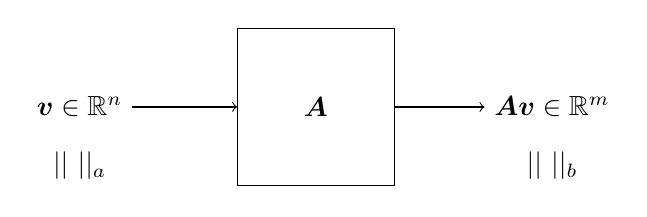
\begin{tikzpicture}
                        \node (v) at (0, 0) {$\vec{v} \in \mathbb{R}^n$};
                        \node at (0, -0.75) {$||\ ||_a$};
                        \node (av) at (6, 0) {$\mat{A} \vec{v} \in \mathbb{R}^m$};
                        \node at (6, -0.75) {$||\ ||_b$};
                        \node at (3, 0) {$\mat{A}$};
                        \draw
                        (v) edge[->] (2, 0)
                        (4, 0) edge[->] (av)
                        (2, 1) -- (4, 1) -- (4, -1) -- (2, -1) -- cycle;
                    \end{tikzpicture}
                    \medskip

                    $|| \mat{A} \vec{v} ||_b \leq || \mat{A} || || \vec{v} ||_a$
                \end{center}
                For the following example, take $(a_{i, j}) = \mat{A} \in \mathbb{R}^{m \times n}$;
                \begin{align*}
                    a_j & = \begin{bmatrix}
                        a_{1, j} \\ a_{2, j} \\ \vdots \\ a_{m, j}
                    \end{bmatrix} & \text{the $j^\text{th}$ column of $\mat{A}$} \\
                    a^i & = \begin{bmatrix}
                        a_{i, 1} & a_{i, 2} & \cdots & a_{i, n}
                    \end{bmatrix} & \text{the $i^\text{th}$ row of $\mat{A}$}
                \end{align*}
                We have the following norms on matrices;
                \begin{align*}
                    || \mat{A} ||_1 & = \max \{|| a_j ||_1 : 1 \leq j \leq n \} \\
                    || \mat{A} ||_\infty & = \max \{|| (a^i)^\top ||_1 : 1 \leq i \leq m \} \\
                    || \mat{A} ||_F & = \sqrt{\summation{i = 1}{m} \summation{j = 1}{n} | a_{i, j} |^2} & \text{Frobenius norm} \\
                    || \mat{A} ||_2 & = \text{largest singular value of } \mat{A} \\
                    \text{let } \mat{A} & = \begin{bmatrix}
                        2 & 3 & 1 & 4 \\
                        1 & 3 & -1 & 5 \\
                        \sqrt{2} & 0 & -2 & 2
                    \end{bmatrix} \\
                    || \mat{A} ||_1 & = \max \{ 3 + \sqrt{2}, 6, 4, 11 \}
                    \\
                    & = 11 \\
                    || \mat{A} ||_\infty & = \max \{ 10, 10, 4 + \sqrt{2} \} \\
                    & = 10 \\
                    || \mat{A} ||_F & = \sqrt{4 + 9 + 1 + 16 + 1 + 9 + 1 + 25 + 2 + 0 + 4 + 4} \\
                    & = 2 \sqrt{19}
                \end{align*}
                Let there be two vector norms, $||\ ||_a$ on $\mathbb{R}^n$ and $||\ ||_b$ on $\mathbb{R}$.
                If $||\ ||$ (matrix norm) satisfies
                \begin{center}
                    $\forall \mat{A} \in \mathbb{R}^{m \times n}, x \in \mathbb{R}^n\ [|| \mat{A}\vec{x} ||_b \leq || \mat{A} || || \vec{x} ||_a]$
                \end{center}
                then $||\ ||$ is \textbf{consistent} with $||\ ||_a$ and $||\ ||_b$.
                Additionally if $a = b$, then $||\ ||$ is \textbf{compatible} with $||\ ||_a$.
                This gives us the following propositions;
                \begin{itemize}
                    \itemsep0em
                    \item $||\ ||_1$ (matrix norm) is compatible with $||\ ||_1$ (vector norm)
                    \item $||\ ||_2$ (matrix norm) is compatible with $||\ ||_2$ (vector norm)
                    \item $||\ ||_\infty$ (matrix norm) is compatible with $||\ ||_\infty$ (vector norm)
                    \item $||\ ||_F$ (matrix norm) is compatible with $||\ ||_2$ (vector norm) $\Rightarrow || \mat{A}\vec{x} ||_2 \leq || \mat{A} ||_F || \vec{x} ||_2$
                \end{itemize}
                Given a vector norm $||\ ||$ on $\mathbb{R}^n$ then the matrix norm $||\ ||$ subordinate to vector norm $||\ ||$ is defined by
                \begin{center}
                    $|| \mat{A} || = \max \{ || \mat{A}\vec{x} || : || \vec{x} || \leq 1 \} \violet{\ = \max \{ || \mat{A}\vec{x} || : || \vec{x} || = 1 \} = \max \{ || \mat{A}\frac{\vec{x}}{|| \vec{x} ||} || : \vec{x} \neq \vec{0} \}}$
                \end{center}
                Using this, we can prove property (iii) (see above).
                We claim that $|| \mat{A} + \mat{B} || \leq || \mat{A} || + || \mat{B} ||$ for matrix norm $||\ ||$ subordinate to vector norm $||\ ||$.
                \begin{align*}
                    || \mat{A} + \mat{B} || & = \max \{ || (\mat{A} + \mat{B})\vec{x} || : || \vec{x} || \leq 1 \} \\
                    & = \max \{ || \mat{A}\vec{x} + \mat{B}\vec{x} || : || \vec{x} || \leq 1 \} \\
                    & \leq \max \{ || \mat{A}\vec{x} || + || \mat{B}\vec{x} || : || \vec{x} || \leq 1 \} & \text{triangle inequality for $||\ ||$} \\
                    & \leq \max \{ || \mat{A}\vec{x} || : || \vec{x} || \leq 1 \} + \max \{ || \mat{B}\vec{x} || : || \vec{x} || \leq 1 \} & \text{maximise independently} \\
                    & = || \mat{A} || + || \mat{B} || & \blacksquare
                \end{align*}
                We are also able to prove property (iv), which we claim to be $|| \mat{B}\mat{A} || \leq || \mat{B} || || \mat{A} ||$.
                \begin{align*}
                    || \mat{B}\mat{A} || & = \max \{ || \mat{B}\mat{A}\vec{x} || : || \vec{x} || \leq 1 \} \\
                    || \mat{B}\mat{A}\vec{x} || & = || \mat{B}(\mat{A}\vec{x}) || \\
                    || \mat{A}\vec{x} || & \leq || \mat{A} || || \vec{x} || & \text{matrix norm subordinate to vector norm}
                    \intertext{
                        To show the line above, we consider the two cases, $\vec{x} \neq \vec{0}$ and $\vec{x} = \vec{0}$.
                        If $\vec{x} = \vec{0}$, no work needs to be done, as it is trivial.
                        I have no idea why this works, but he wrote it.
                    }
                    \text{show } \left|\left| \mat{A}\frac{\vec{x}}{|| \vec{x} ||} \right|\right| & \leq || \mat{A} || \\
                    \text{but } \left|\left| \frac{\vec{x}}{|| \vec{x} ||} \right|\right| & = 1 & \Rightarrow \\
                    || \mat{A}\vec{x} || & \leq || \mat{A} || || \vec{x} ||
                    \intertext{Continuing on, we have}
                    || \mat{B}\mat{A}\vec{x} || & = || \mat{B}(\mat{A}\vec{x}) || \\
                    & \leq || \mat{B} || || \mat{A}\vec{x} || \\
                    & \leq || \mat{B} || || \mat{A} || || \vec{x} || \\
                    || \mat{B}\mat{A} || & = \max \{ || \mat{B}\mat{A}\vec{x} || : || \vec{x} || \leq 1 \} \\
                    & \leq \max \{ || \mat{B} || || \mat{A} || || \vec{x} || : || \vec{x} || \leq 1 \} \\
                    & = || \mat{B} || || \mat{A} || \max \{ || \vec{x} || : || \vec{x} || \leq 1 \} & \text{obviously 1, as bounded on top}\\
                    & = || \mat{B} || || \mat{A} || & \blacksquare
                \end{align*}
            \subsubsection*{Complex Vectors}
                \begin{align*}
                    \mathbb{C}^n & = \left\{ \vec{v} = \begin{bmatrix}
                        v_1 \\ \vdots \\ v_n
                    \end{bmatrix} : v_i \in \mathbb{C} \right\} \\
                    z \in \mathbb{C} & = a + ib & a \in \mathbb{R}, b \in \mathbb{R}, i = \sqrt{-1} \\
                    z^* & = a - ib \\
                    | z | & = \sqrt{a^2 + b^2}
                \end{align*}
                Take a linear map $f : \mathbb{C}^n \to \mathbb{C}^m$, the same properties hold;
                \begin{align*}
                    f(a \vec{v} + b \vec{w}) & = af(\vec{v}) + bf(\vec{w}) & a, b \in \mathbb{C}
                \end{align*}
                We also want to define something similar to the dot product in $\mathbb{R}^n$;
                \begin{align*}
                    \vec{v} \cdot \vec{w} & = || \vec{v} ||_2 || \vec{w} ||_2 \cos \theta_{\vec{v},\vec{w}} \\
                    \vec{v} \cdot \vec{v} & = \sqrt{|| \vec{v} ||_2^2} \\
                    & = || \vec{v} ||_2 \\
                    <\vec{v}, \vec{w}> & = \summation{i = 1}{n} v_i^* w_i \\
                    <\vec{v}, \vec{v}> & = \summation{i = 1}{n} v_i^* v_i \\
                    & = \summation{i = 1}{n} | v_i |^2
                \end{align*}
                The standard basis in $\mathbb{R}^n$ is defined as $(\vec{e_1}, \dots, \vec{e_n})$ where
                \begin{center}
                    $\vec{e_j} = \begin{bmatrix}
                        0 \\ 0 \\ \vdots \\ 1 \\ \vdots \\ 0
                    \end{bmatrix} \begin{matrix}
                        1^\text{st} \\ 2^\text{nd} \\ \vdots \\ j^\text{th} \\ \vdots \\ n^\text{th}
                    \end{matrix}$
                \end{center}
                For any vector $\vec{v} \in \mathbb{C}^n$, it can be written in the standard basis as such;
                \begin{align*}
                    \vec{v} & = \begin{bmatrix}
                        v_1 \\ \vdots \\ v_n
                    \end{bmatrix} \\
                    & = v_1\vec{e_1} + \dots + v_n\vec{e_n}
                \end{align*}
            \subsubsection*{Basis Change, Again}
                Let the linear map $f : \mathbb{R}^n \to \mathbb{R}^m$.
                \begin{align*}
                    \mat{B} & = (\vec{b_1}, \dots, \vec{b_n}) & \text{an ordered basis of } \mathbb{R}^n \\
                    \mat{D} & = (\vec{d_1}, \dots, \vec{d_m}) & \text{an ordered basis of } \mathbb{R}^m
                \end{align*}
                Find the matrix $\mat{A}$ ($\mat{A} := f_{\mat{D}\mat{B}}$)representing $f$ with respect to (?) $\mat{B}$ and $\mat{D}$.
                \begin{align*}
                    \vec{v} & = \begin{bmatrix}
                        v_1 \\ \vdots \\ v_n
                    \end{bmatrix} & \text{coordinates of a point } \vec{p} \in \mathbb{R}^n \\
                    \vec{p} & = \summation{j = 1}{n} v_j \vec{b_j} \\
                    \mat{A}\vec{v} & & \text{should be coordinate of } f(\vec{p}) \in \mathbb{R}^m \\
                    f(\vec{p}) & = \summation{i = 1}{m} (\mat{A}\vec{v})_i \vec{d_i} \\
                    f(\vec{b_j}) \in \mathbb{R}^m & = \summation{i = 1}{m} a_{i, j}\vec{d_i} & 1 \leq j \leq n
                \end{align*}
                Take $\mat{B} \in \mathbb{R}^{m \times n}$, where $\mat{B} = [\vec{b_1}, \vec{b_2}, \dots, \vec{b_n}]$, and $e_1, \dots, \vec{e_m}$ being the standard basis (see previous).
                \begin{align*}
                    \mat{B}\vec{e_j} & = \mat{B} \begin{bmatrix}
                        0 \\ \vdots \\ 0 \\ 1 \\ 0 \\ \vdots \\0
                    \end{bmatrix} \begin{matrix}
                        \phantom{0} \\ \phantom{\vdots} \\ \phantom{0} \\ \leftarrow j^\text{th} \\ \phantom{0} \\ \phantom{\vdots} \\ \phantom{0}
                    \end{matrix} \\
                    & = b_{1, j}\vec{e_1} + ... + b_{m, j}\vec{e_m}
                \end{align*}
                Suppose $m = n$ and also $f = \text{id}$ (identity), but $\mat{B}$ and $\mat{D}$ are different.
                The matrix $(\text{id})_{\mat{D} \mat{B}}$ represents a change of basis from $\mat{B}$ to $\mat{D}$.
                The point $\vec{p} \in \mathbb{R}^n$ has coordinates $\vec{x} \in \mathbb{R}^n$ with respect to $\mat{B}$, and $\vec{y} \in \mathbb{R}^n$ with respect to $\mat{D}$.
                \begin{center}
                    $\mat{D}\vec{y} = \vec{p} = \mat{B}\vec{x} = x_1\vec{b_1} + \dots + x_n\vec{b_n}$
                \end{center}
                From this we gather $\mat{D}\vec{y} = \mat{B}\vec{x}$, therefore $\vec{y} = \mat{D}^{-1}\mat{B}\vec{x} = (\text{id})_{\mat{D}\mat{B}}\vec{x}$, which means that
                \begin{center}
                    $(\text{id})_{\mat{D}\mat{B}} = \mat{D}^{-1}\mat{B}$
                \end{center}
                Some stuff on functions between bases?
                \begin{center}
                    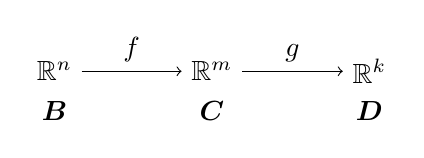
\begin{tikzpicture}
                        \node (rn) at (0, 0) {$\mathbb{R}^n$};
                        \node (rm) at (2, 0) {$\mathbb{R}^m$};
                        \node (rk) at (4, 0) {$\mathbb{R}^k$};
                        \node (b) at (0, -0.5) {$\mat{B}$};
                        \node (c) at (2, -0.5) {$\mat{C}$};
                        \node (d) at (4, -0.5) {$\mat{D}$};

                        \draw
                        (rn) edge[->] node[above]{$f$} (rm)
                        (rm) edge[->] node[above]{$g$} (rk);
                    \end{tikzpicture}
                    \\
                    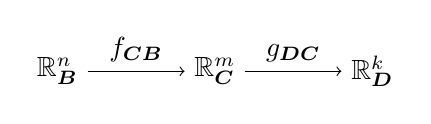
\begin{tikzpicture}
                        \node (rnb) at (0, 0) {$\mathbb{R}_{\mat{B}}^n$};
                        \node (rmc) at (2, 0) {$\mathbb{R}_{\mat{C}}^m$};
                        \node (rkd) at (4, 0) {$\mathbb{R}_{\mat{D}}^k$};

                        \draw
                        (rnb) edge[->] node[above]{$f_{\mat{C}\mat{B}}$} (rmc)
                        (rmc) edge[->] node[above]{$g_{\mat{D}\mat{C}}$} (rkd);
                    \end{tikzpicture}
                    \\
                    $g_{\mat{D}\mat{C}}f_{\mat{C}\mat{B}} = (g \circ f)_{\mat{D}\mat{B}}$
                \end{center}
                This then goes into change of basis, but see last year's \textbf{CO145}.
        \subsection*{22nd January 2020}
            \subsubsection*{Tutorial Question}
                $f : \mathbb{R}^2 \to \mathbb{R}^2$ is a linear map, and $\mat{E} = (\vec{e_1}, \vec{e_2})$ is an ordered basis.
                \begin{align*}
                    f(\vec{e_1}) & = 5\vec{e_1} - 6\vec{e_2} \\
                    f(\vec{e_2}) & = 3\vec{e_1} + \vec{e_2}
                \end{align*}
                We only care about what the linear map does to the ordered basis, as anything else can be done by linearity.
                \begin{enumerate}[(i)]
                    \itemsep0em
                    \item Find $f_{\mat{E}\mat{E}}$, the matrix representation of $f$ in $\mat{E}$ - note that this has the same input space as the output space, but it can be different.
                        \medskip

                        The first column can be done by reading the entry for for $f(\vec{e_1})$, and similarly for the second column as follows;
                        \begin{center}
                            $f_{\mat{E}\mat{E}} = \begin{bmatrix}
                                5 & 3 \\
                                -6 & 1
                            \end{bmatrix}$
                        \end{center}
                    \item If we have another ordered basis $\mat{D} = (\vec{d_1}, \vec{d_2})$, where $\vec{d_1} = \vec{e_1} - \vec{e_2}$ and $\vec{d_2} = \vec{e_1} + \vec{e_2}$, find $f_{\mat{D}\mat{D}}$.
                        \begin{center}
                            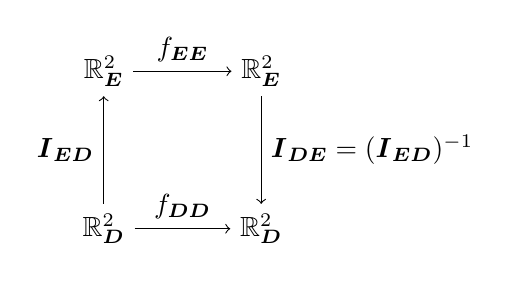
\begin{tikzpicture}
                                \node (rel) at (0, 0) {$\mathbb{R}_{\mat{E}}^2$};
                                \node (rer) at (2, 0) {$\mathbb{R}_{\mat{E}}^2$};
                                \node (rdl) at (0, -2) {$\mathbb{R}_{\mat{D}}^2$};
                                \node (rdr) at (2, -2) {$\mathbb{R}_{\mat{D}}^2$};

                                \draw
                                (rdl) edge[->] node[left]{$\mat{I}_{\mat{E}\mat{D}}$} (rel)
                                (rel) edge[->] node[above]{$f_{\mat{E}\mat{E}}$} (rer)
                                (rer) edge[->] node[right] {$\mat{I}_{\mat{D}\mat{E}} = (\mat{I}_{\mat{E}\mat{D}})^{-1}$} (rdr)
                                (rdl) edge[->] node[above]{$f_{\mat{D}\mat{D}}$} (rdr);
                            \end{tikzpicture}
                        \end{center}
                        $\mat{I}_{\mat{E}\mat{D}}$ can easily be obtained by reading the entries for $\vec{d_1}$ for the first column, and similarly for $\vec{d_2}$ in the second column;
                        \begin{align*}
                            \mat{I}_{\mat{E}\mat{D}} & = \begin{bmatrix}
                                1 & 1 \\
                                -1 & 1
                            \end{bmatrix} \\
                            \mat{I}_{\mat{D}\mat{E}} & = (\mat{I}_{\mat{E}\mat{D}})^{-1} \\
                            & = \frac{1}{2} \begin{bmatrix}
                                1 & -1 \\
                                1 & 1
                            \end{bmatrix} \\
                            f_{\mat{D}\mat{D}} & = \mat{I}_{\mat{D}\mat{E}} f_{\mat{E}\mat{E}} \mat{I}_{\mat{E}\mat{D}} \\
                            & = \frac{1}{2} \begin{bmatrix}
                                1 & -1 \\
                                1 & 1
                            \end{bmatrix} \begin{bmatrix}
                                5 & 3 \\
                                -6 & 1
                            \end{bmatrix} \begin{bmatrix}
                                1 & 1 \\
                                -1 & 1
                            \end{bmatrix} \\
                            & = \frac{1}{2} \begin{bmatrix}
                                1 & 13 \\
                                -5 & 3
                            \end{bmatrix}
                        \end{align*}
                \end{enumerate}
            \subsubsection*{Eigenvalues + Generalised Eigenvectors}
                Working with a matrix $\mat{A} \in \mathbb{C}^{m \times m}$.
                For an eigenvector $\vec{v} \in \mathbb{C}^m \setminus \{ \vec{0} \}$, and an eigenvalue $\lambda \in \mathbb{C}$, $\mat{A}\vec{v} = \lambda\vec{v} \Rightarrow (\mat{A} - \lambda\mat{I})\vec{v} = \vec{0} \Rightarrow | \mat{A} - \lambda\mat{I} | = 0 \Rightarrow P_{\mat{A}}(\lambda) = 0$ (characteristic polynomial).
                This complex polynomial will be of degree $m$, and it will have precisely $m$ roots (including multiplicity).
                Suppose $P_{\mat{A}}(\lambda) = 0$, then $(\mat{A} - \lambda\mat{I})\vec{v} = \vec{0}$ has a solution where $\vec{v} \neq \vec{0}$.
                \medskip

                Assume we have $\lambda_1, \dots, \lambda_t$ distinct eigenvalues, meaning that $P_{\mat{A}}(\lambda_i) = 0$ for $1 \leq i \leq t$.
                This means we can write the characteristic polynomial as;
                \begin{center}
                    $P_{\mat{A}}(\lambda) = (\lambda - \lambda_1)^{m_1}(\lambda - \lambda_2)^{m_2} \dots (\lambda - \lambda_t)^{m_t}$
                \end{center}
                Where $m_i$ is the \textbf{algebraic multiplicity} of $\lambda_i$. $m_i \in \mathbb{N}$, and also $1 \leq m_i \leq m$, as it must not exceed the dimension of the matrix.
                On the other hand, the \textbf{geometric multiplicity} of $\lambda_i$ is $\ell_i$, which is the \textbf{nullity} of $(\mat{A} - \lambda_i\mat{I})$.
                The nullity is the dimension of the kernel / null-space. $1 \leq \ell_i \leq m_i$, as we already have at least one non-zero solution from $(\mat{A} - \lambda_i\mat{I})\vec{v} = \vec{0}$.
                \medskip

                In the nice case, we have $\ell_i = m_i$, for $1 \leq i \leq t$, which means the matrix is diagonalisable.
                We have $m_i$ linearly independent vectors $(\vec{v_{i, 1}}, \vec{v_{i, 2}, \dots, \vec{v_{i, m_i}}})$ which satisfy
                \begin{center}
                    $\mat{A}\vec{v_{i, j}} = \lambda_i\vec{v_{i, j}}$ for $1 \leq j \leq m_i$
                \end{center}
                If we take these eigenvectors as an ordered basis;
                \begin{center}
                    $\mat{B} = [\vec{v_{1, 1}}, \vec{v_{1, 2}}, \dots, \vec{v_{1, m_1}}, \vec{v_{2, 1}}, \vec{v_{2, 2}}, \dots, \vec{v_{2, m_2}}, \dots \vec{v_{t, 1}}, \vec{v_{t, 2}}, \dots, \vec{v_{t, m_t}}]$
                \end{center}
                We also want to note that $\summation{i = 1}{t} m_i = m$, as that is the degree of the characteristic polynomial.
                Multiplying the basis by the original matrix, we get;
                \begin{center}
                    $\mat{A}\mat{B} = [\lambda_1\vec{v_{1, 1}}, \lambda_1\vec{v_{1, 2}}, \dots, \lambda_1\vec{v_{1, m_1}}, \lambda_2\vec{v_{2, 1}}, \lambda_2\vec{v_{2, 2}}, \dots, \lambda_2\vec{v_{2, m_2}}, \dots \lambda_t\vec{v_{t, 1}}, \lambda_t\vec{v_{t, 2}}, \dots, \lambda_t\vec{v_{t, m_t}}]$
                \end{center}
                Since all the columns of $\mat{B}$ are linearly independently, by our definition, the inverse $\mat{B}^{-1}$ exists.
                Therefore, we can write
                \begin{center}
                    $\mat{B}^{-1}\mat{A}\mat{B} = \begin{bmatrix}
                        \lambda_1 \\
                        & \ddots \\
                        & & \lambda_1 \\
                        & & & \lambda_2 \\
                        & & & & \ddots \\
                        & & & & & \lambda_2 \\
                        & & & & & & \ddots \\
                        & & & & & & & \lambda_t \\
                        & & & & & & & & \ddots \\
                        & & & & & & & & & \lambda_t
                    \end{bmatrix}$
                    (everything else is 0)
                \end{center}
                Which has $m_1$ instances of $\lambda_1$, followed by $m_2$ instances of $\lambda_2$, and so on, until $m_t$ instances of $\lambda_t$.
            \subsubsection*{Example for $\ell_i = m_i$}
                \begin{align*}
                    \mat{A} & = \begin{bmatrix}
                        4 & 0 & 1 \\
                        2 & 3 & 2 \\
                        1 & 0 & 4
                    \end{bmatrix} \\
                    | \mat{A} - \lambda\mat{I} | & = (\lambda - 3)^2(\lambda - 5) \\
                    \lambda_1 & = 3 & \text{two linearly independently eigenvectors} \\
                    \vec{v_{1, 1}} & = \begin{bmatrix}
                        0 \\ 1 \\ 0
                    \end{bmatrix} \\
                    \vec{v_{1, 2}} & = \begin{bmatrix}
                        -1 \\ 0 \\ 1
                    \end{bmatrix} \\
                    \lambda_2 & = 5 \\
                    \vec{v_{2, 1}} & = \begin{bmatrix}
                        1 \\ 2 \\ 1
                    \end{bmatrix} \displaybreak \\
                    \mat{B} & = \begin{bmatrix}
                        0 & -1 & 1 \\
                        1 & 0 & 2 \\
                        0 & 1 & 1
                    \end{bmatrix} \\
                    \mat{B}^{-1} & = \frac{1}{2} \begin{bmatrix}
                        -2 & 2 & -2 \\
                        -1 & 0 & 1 \\
                        1 & 0 & 1
                    \end{bmatrix} \\
                    \mat{B}^{-1}\mat{A}\mat{B} & = \begin{bmatrix}
                        3 & 0 & 0 \\
                        0 & 3 & 0 \\
                        0 & 0 & 5
                    \end{bmatrix}
                \end{align*}
            \subsubsection*{Trivial Example for $\ell_i < m_i$}
                \begin{align*}
                    \mat{A} & = \begin{bmatrix}
                        0 & 0 \\
                        0 & 1
                    \end{bmatrix} \\
                    | \mat{A} - \lambda\mat{I} | & = \lambda^2 \\
                    \lambda_1 & = 0 \\
                    \vec{v_1} & = \begin{bmatrix}
                        1 \\ 0
                    \end{bmatrix} & \text{only solution, hence } \ell_1 = 1 < 2 = m_1 \\
                    (\mat{A} - 0\mat{I}) \begin{bmatrix}
                        0 \\ 1
                    \end{bmatrix} & = \begin{bmatrix}
                        0 & 0 \\
                        0 & 1
                    \end{bmatrix} \begin{bmatrix}
                        0 \\ 1
                    \end{bmatrix} \\
                    & = \begin{bmatrix}
                        1 \\ 0
                    \end{bmatrix}
                    \intertext{although this vector is not mapped to zero, it is mapped to something that \textbf{will} be mapped to zero}
                    (\mat{A} - 0\mat{I})^2 \begin{bmatrix}
                        0 \\ 1
                    \end{bmatrix} & = (\mat{A} - 0\mat{I}) (\mat{A} - 0\mat{I}) \begin{bmatrix}
                        0 \\ 1
                    \end{bmatrix} \\
                    & = (\mat{A} - 0\mat{I}) \begin{bmatrix}
                        1 \\ 0
                    \end{bmatrix} \\
                    & = \vec{0}
                \end{align*}
                We say $\begin{bmatrix}
                    0 \\ 1
                \end{bmatrix}$ is a generalised eigenvector for $\lambda_1 = 0$.
                A vector which is not mapped by $(\mat{A} - \lambda\mat{I})$ to $\vec{0}$, but is $\vec{0}$ when iterated once more.
            \subsubsection*{Less Trivial Example}
                \begin{align*}
                    \mat{A} & = \begin{bmatrix}
                        1 & 1 & 1 \\
                        0 & 1 & 0 \\
                        0 & 0 & 1
                    \end{bmatrix} \\
                    | \mat{A} - \lambda\mat{I} | & = (1 - \lambda)^3 \\
                    \lambda_1 & = 1 & m_1 = 3 \\
                    (\mat{A} - \mat{I})\vec{x} & = \vec{0} & \Leftrightarrow \\
                    \begin{bmatrix}
                        0 & 1 & 1 \\
                        0 & 0 & 0 \\
                        0 & 0 & 0
                    \end{bmatrix} \vec{x} & = \vec{0}
                    \intertext{this has rank 1, and therefore by rank-nullity theorem (rank + nullity = 3), has 2 linearly independent solutions, therefore $\ell_1 = 2 < 3 = m_1$}
                    \vec{v_1} & = \begin{bmatrix}
                        0 \\ 1 \\ -1
                    \end{bmatrix} \displaybreak \\
                    \vec{v_2} & = \begin{bmatrix}
                        1 \\ 0 \\ 0
                    \end{bmatrix}
                    \intertext{to find the generalised eigenvector $\vec{v_3}$, we want to find some vector that is mapped by $(\mat{A} - 1 \mat{I})$ to the eigenspace, which is some linear combination of $\vec{v_1}$ and $\vec{v_2}$}
                    (\mat{A} - \mat{I}) \vec{v_3} & = \alpha_1 \vec{v_1} + \alpha_2 \vec{v_2} & \Leftrightarrow \\
                    \begin{bmatrix}
                        0 & 1 & 1 \\
                        0 & 0 & 0 \\
                        0 & 0 & 0
                    \end{bmatrix} \begin{bmatrix}
                        x_1 \\ x_2 \\ x_3
                    \end{bmatrix} & = \begin{bmatrix}
                        0 \\ \alpha_1 \\ -\alpha_1
                    \end{bmatrix} + \begin{bmatrix}
                        \alpha_2 \\ 0 \\ 0
                    \end{bmatrix} \\
                    & = \begin{bmatrix}
                        x_2 + x_3 \\ 0 \\ 0
                    \end{bmatrix} & \Leftrightarrow \\
                    \alpha_1 & = 0 \\
                    x_2 + x_3 & = \alpha_2 & \text{let } x_2 = 0 \Rightarrow x_3 = \alpha_2 = 1 \\
                    \vec{v_3} & = \begin{bmatrix}
                        0 \\ 0 \\ 1
                    \end{bmatrix} \\
                    \mat{B} & = [\vec{v_1}, \vec{v_2}, \vec{v_3}] \\
                    & = \begin{bmatrix}
                        0 & 1 & 0 \\
                        1 & 0 & 0 \\
                        -1 & 0 & 1
                    \end{bmatrix} \\
                    \mat{B}^{-1}\mat{A}\mat{B} & = \begin{bmatrix}
                        1 & 0 & 0 \\
                        0 & 1 & 1 \\
                        0 & 0 & 1
                    \end{bmatrix} & \text{the extra 1 is from $\vec{v_2}$?}
                \end{align*}
                This is in Jordan Normal Form.
                For some $\lambda_i$ eigenvalue, and $\ell_i \leq m_i$, the sum of the sizes of the blocks is $m_i$, and the number of blocks is $\ell_i$.
                If $\lambda_i$ is an eigenvalue of $\mat{A}$ with algebraic multiplicity $m_i$, then the nullity of $(\mat{A} - \lambda_i \mat{I})^{m_i} = m_i$.
                \medskip

                \textbf{Definition}: $\vec{v} \in \mathbb{R}^m$ is a generalised eigenvector for $\lambda_i$ if $(\mat{A} - \lambda_i \mat{I})^{m_i} \vec{v} = \vec{0}$.
                The maximum iterations is $m_i$, but can be less.
        \subsection*{23rd January 2020}
            In general;
            \begin{itemize}
                \itemsep0em
                \item $\forall j\ [\ell_j = m_j] \Rightarrow \mat{A}$ is diagonalisable
                \item $\exists j\ [\ell_j < m_j] \Rightarrow \mat{A}$ is diagonalisable or \textbf{almost} diagonalisable
            \end{itemize}
            The following is a very poor explanation of what the form looks like, because I don't know how to draw blocks in \LaTeX.
            See Panopto at timestamp 13:17 for a proper drawing.
            \begin{align*}
                \mat{A} & = \begin{bmatrix}
                    \mat{B_{\lambda_1}} \\
                    & \ddots \\
                    & & \mat{B_{\lambda_t}}
                \end{bmatrix} \\
                \mat{B_j} & = \begin{bmatrix}
                    \mat{J_j} \\
                    & \ddots \\
                    & & \mat{J_j}
                \end{bmatrix} & \text{all $\mat{J_j}$ can be of different sizes, $\mat{B_j} \in \mathbb{R}^{m_j \times m_j}$} \displaybreak \\
                \mat{J_i} & = \begin{bmatrix}
                    \lambda_i & 1 \\
                    & \lambda_i & \ddots \\
                    & & \ddots & 1 \\
                    & & & \lambda_i
                \end{bmatrix}
            \end{align*}
            \subsubsection*{Spectral Decomposition of Symmetric Matrices}
                In almost all areas of computer science, symmetric matrices are the dominant paradigm.
                All the eigenvalues of real symmetric matrices are real, and are always diagonalisable.
                A symmetric matrix is always a square matrix $\mat{A} \in \mathbb{R}^{n \times n}$, which also satisfies $\mat{A}^\top = \mat{A}$, meaning it is symmetric along the diagonal (the elements above the diagonal determine the elements below, and vice versa).
                We are to prove the following properties;
                \begin{enumerate}[(i)]
                    \itemsep0em
                    \item All eigenvalues of $\mat{A}$ are real.
                        \medskip

                        First assume that $\vec{v} \in \mathbb{C}^n$, as we don't yet know that it is real, therefore we can have the case $\lambda \in \mathbb{C}$.
                        \begin{align*}
                            \mat{A}\vec{v} & = \lambda\vec{v} & \Rightarrow \\
                            \vec{v}^{*^\top}\mat{A}\vec{v} & = \lambda \vec{v}^{*^\top}\vec{v} \\
                            & = \lambda || \vec{v} ||^2 & (1) \\
                            \vec{v}^{*^\top}\mat{A}\vec{v} & = \left(\vec{v}^{*^\top}\mat{A}\right)\vec{v} \\
                            & = \left((\mat{A}\vec{v})^\top\right)^* \vec{v}
                            \intertext{briefly proving the above;}
                            \left((\mat{A}\vec{v})^\top\right)^* & = \left(\vec{v}^\top\mat{A}^\top\right)^* & \text{taking the transpose inside the bracket} \\
                            & = \left(\vec{v}^\top\right)^* \mat{A}^* & \text{taking the conjugate inside and $\mat{A}^\top = \mat{A}$} \\
                            & = \left(\vec{v}^\top\right)^* \mat{A} & \text{$\mat{A}$ is real valued matrix}
                            \intertext{continuing on;}
                            & = \left((\lambda\vec{v})^\top\right)^* \vec{v} & \text{$\vec{v}$ is an eigenvector} \\
                            & = \lambda^* \left(\vec{v}^\top\right)^* \vec{v} & \text{transposing a scalar does nothing} \\
                            & = \lambda^* || \vec{v} ||^2 & (2)
                        \end{align*}
                        By comparing results, $(1) = (2)$, hence $\lambda^* = \lambda$ (dividing through by $|| \vec{v} ||^2$ is allowed, since we know it is non-zero by properties of vector norms, and $\vec{v} \neq \vec{0}$ by properties of eigenvectors).
                        As the complex conjugate of $\lambda$ is the same as $\lambda$, we can conclude that $\lambda \in \mathbb{R}$.
                    \item Eigenvectors corresponding to different eigenvalues of $\mat{A}$ are perpendicular.
                        \medskip

                        Note that with the above result, we know that $\vec{v} \in \mathbb{R}^n$, as there is no possible way to obtain complex values with a real valued matrix and a real valued eigenvalue.
                        \begin{align*}
                            \mat{A}\vec{v_1} & = \lambda_1 \vec{v_1} \\
                            \mat{A}\vec{v_2} & = \lambda_2 \vec{v_2} \\
                            \lambda_1 & \neq \lambda_2 \\
                            \vec{v_2}^\top\mat{A}\vec{v_1} & = \lambda_1 \vec{v_2}^\top \vec{v_1} \\
                            & = \lambda_1 (\vec{v_1} \cdot \vec{v_2}) & (1) \\
                            \vec{v_2}^\top\mat{A}\vec{v_1} & = \left(\vec{v_2}^\top\mat{A}\right)\vec{v_1} \\
                            & = (\mat{A}\vec{v_2})^\top\vec{v_1} & \text{adding a transpose and $\mat{A}^\top = \mat{A}$} \\
                            & = \lambda_2 \vec{v_2}^\top \vec{v_1} & \text{$\vec{v_2}$ is an eigenvector} \\
                            & = \lambda_2 (\vec{v_1} \cdot \vec{v_2}) & (2)
                        \end{align*}
                        Similarly, comparing results (1) and (2), we get
                        \begin{align*}
                            \lambda_1 (\vec{v_1} \cdot \vec{v_2}) & = \lambda_2 (\vec{v_1} \cdot \vec{v_2}) & \Leftrightarrow \\
                            \lambda_1 (\vec{v_1} \cdot \vec{v_2}) - \lambda_2 (\vec{v_1} \cdot \vec{v_2}) & = 0 \\
                            (\lambda_1 - \lambda_2)(\vec{v_1} \cdot \vec{v_2}) & = 0 & \Leftrightarrow \\
                            \lambda_1 & = \lambda_2 \\
                            \text{or } \vec{v_1} \cdot \vec{v_2} & = 0
                        \end{align*}
                        The former is not possible due to the condition that they are different eigenvalues, therefore $\vec{v_1} \cdot \vec{v_2} = 0$.
                        As neither are the zero vector, by definition of eigenvectors, $\cos \theta = 0$, therefore they are perpendicular.
                    \item (Tutorial 3) If $\lambda_j$ is an eigenvalue of $\mat{A}$ then $\ell_j = m_j$, therefore $\mat{A}$ is diagonalisable.
                        \medskip

                        Come back to this in two weeks?
                \end{enumerate}
                To conclude, we get all the eigenvectors and we normalise them (divide by the $\ell_2$-norm), and we can assume they are pairwise orthogonal.
                There is an orthonormal basis for $\mathbb{R}^n$ consisting of eigenvectors of $\mathbb{A}$; $(\vec{v_1}, \dots, \vec{v_n})$, where $\vec{v_j} \in \mathbb{R}^n$.
                This has the following properties;
                \begin{itemize}
                    \itemsep0em
                    \item $\mat{A}\vec{v_j} = \lambda_j \vec{v_j}$
                    \item $\vec{v_i} \bot \vec{v_j}$, when $i \neq j$ \hfill perpendicular
                    \item $|| \vec{v_i} || = 1$ for $i = 1, \dots, n$
                \end{itemize}
            \subsubsection*{Examples}
                For an example in $\mathbb{R}^{2 \times 2}$;
                \begin{align*}
                    \mat{A} & = \begin{bmatrix}
                        1 & 2 \\
                        2 & 1
                    \end{bmatrix} \\
                    | \mat{A} - \lambda\mat{I} | & = (1 - \lambda)^2 - 4 \\
                    \lambda_1 & = 3 \\
                    \lambda_2 & = -1 \\
                    \vec{v_1} & = \frac{1}{\sqrt{2}} \begin{bmatrix}
                        1 \\ 1
                    \end{bmatrix} & \text{normalise straight away} \\
                    \vec{v_2} & = \frac{1}{\sqrt{2}} \begin{bmatrix}
                        1 \\ -1
                    \end{bmatrix} \\
                    \mat{V} & = [\vec{v_1}, \vec{v_2}] & \text{orthonormal basis of } \mathbb{R}^2 \\
                    & = \frac{1}{\sqrt{2}} \begin{bmatrix}
                        1 & 1 \\
                        1 & -1
                    \end{bmatrix} \\
                    \mat{A}\mat{V} & = [\mat{A}\vec{v_1}, \mat{A}\vec{v_2}] \\
                    & = [3 \vec{v_1}, - \vec{v_2}]
                    \intertext{For a symmetric matrix, if we have a matrix $\mat{V}$ representing the orthonormal basis of the eigenvectors, $\mat{V}^{-1} = \mat{V}^\top$}
                    \mat{V}^{-1}\mat{A}\mat{V} & = \mat{V}^\top\mat{A}\mat{V} \\
                    & = \mat{V}^\top [3 \vec{v_1}, - \vec{v_2}] \\
                    & = \begin{bmatrix}
                        \vec{v_1}^\top \\
                        \vec{v_2}^\top
                    \end{bmatrix} [3 \vec{v_1}, - \vec{v_2}] \\
                    & = \begin{bmatrix}
                        3 & 0 \\
                        0 & -1
                    \end{bmatrix} & \text{dot product with unit length ($\vec{v_1} \bot \vec{v_2}$)}
                \end{align*}
                For an example in $\mathbb{R}^{3 \times 3}$;
                \begin{align*}
                    \mat{A} & = \begin{bmatrix}
                        1 & 1 & 3 \\
                        1 & 3 & 1 \\
                        3 & 1 & 1
                    \end{bmatrix}
                    \intertext{now he just shows some intuition on getting an eigenvalue?}
                    | \mat{A} - \lambda\mat{I} | & = \begin{vmatrix}
                        1 - \lambda & 1 & 3 \\
                        1 & 3 - \lambda & 1 \\
                        3 & 1 & 1 - \lambda
                    \end{vmatrix} \\
                    & = \begin{vmatrix}
                        5 - \lambda & 1 & 3 \\
                        5 - \lambda & 3 - \lambda & 1 \\
                        5 - \lambda & 1 & 1 - \lambda
                    \end{vmatrix} & \vec{c_1}^\prime = \vec{c_1} + \vec{c_2} + \vec{c_3} \\
                    & = 0 \\
                    \lambda_1 & = 5 \\
                    \text{trace}(\mat{A}) & = \lambda_1 + \lambda_2 + \lambda_3 \\
                    & = 5 & \Rightarrow \\
                    \lambda_2 + \lambda_3 & = 0 \\
                    | \mat{A} | & = \lambda_1 \lambda_2 \lambda_3 \\
                    & = -20 & \Rightarrow \\
                    \lambda_2 \lambda_3 & = -4 \\
                    \lambda_2 & = 2 \\
                    \lambda_3 & = -2 \\
                    \vec{v_1} & = \frac{1}{\sqrt{3}} \begin{bmatrix}
                        1 \\ 1 \\ 1
                    \end{bmatrix} \\
                    \vec{v_2} & = \frac{1}{\sqrt{6}} \begin{bmatrix}
                        1 \\ -2 \\ 1
                    \end{bmatrix} \\
                    \vec{v_3} & = \frac{1}{\sqrt{2}} \begin{bmatrix}
                        1 \\ 0 \\ 1
                    \end{bmatrix} \\
                    \mat{V} & = [\vec{v_1}, \vec{v_2}, \vec{v_3}] \\
                    \mat{V}^{-1} & = \mat{V}^\top \\
                    \mat{V}^{-1}\mat{A}\mat{V} & = \mat{V}^\top\mat{A}\mat{V} \\
                    & = \begin{bmatrix}
                        5 & 0 & 0 \\
                        0 & 2 & 0 \\
                        0 & 0 & -2
                    \end{bmatrix} & \text{spectral decomposition of a symmetric matrix}
                \end{align*}
            \subsubsection*{Proof of $\mat{V}^{-1} = \mat{V}^\top$}
                We define $\mat{B} \in \mathbb{R}^{n \times n}$ as an \textbf{orthogonal matrix} if all columns $\vec{b_j}$ for $1 \leq j \leq n$ form an orthonormal basis of $\mathbb{R}^n$, such that the two properties hold;
                \begin{itemize}
                    \itemsep0em
                    \item $\vec{b_j} \cdot \vec{b_i} = 0$ when $i \neq j$
                    \item $\vec{b_j} \cdot \vec{b_j} = 1$
                \end{itemize}
                We want to prove that $\mat{B}^{-1} = \mat{B}^\top$:
                \begin{align*}
                    \mat{B} & = [\vec{b_1}, \dots, \vec{b_n}] \\
                    \mat{B}^\top & = \begin{bmatrix}
                        \vec{b_1}^\top \\
                        \vdots \\
                        \vec{b_n}^\top
                    \end{bmatrix} \\
                    \mat{B}^\top\mat{B} & = \begin{bmatrix}
                        \vec{b_1}^\top \\
                        \vdots \\
                        \vec{b_n}^\top
                    \end{bmatrix} [\vec{b_1}, \dots, \vec{b_n}] \\
                    & = \begin{bmatrix}
                        1 & 0 & \cdots & 0 \\
                        0 & 1 & \ddots & \vdots \\
                        \vdots & \ddots & \ddots & 0 \\
                        0 & \cdots & 0 & 1
                    \end{bmatrix} \\
                    & = \mat{I}_n
                \end{align*}
            \subsubsection*{Preservation of Length}
                The length of a vector $\vec{x}$ is preserved under orthogonal transformation;
                \begin{align*}
                    (\mat{V}\vec{x}) \cdot (\mat{V}\vec{x}) & = (\mat{V}\vec{x})^\top (\mat{V}\vec{x}) \\
                    & = \vec{x}^\top \mat{V}^\top \mat{V} \vec{x} \\
                    & = \vec{x}^\top \mat{V}^{-1} \mat{V} \vec{x} \\
                    & = \vec{x}^\top \vec{x} \\
                    & = \vec{x} \cdot \vec{x}
                \end{align*}
            \subsubsection*{Geometric Intuition}
                Take a real symmetric matrix $\mat{A} \in \mathbb{R}^{n \times n}$, such that $\mat{A}^\top = \mat{A}$.
                Assume we have processed it to get the eigenvalues $\lambda_1, \dots, \lambda_n$, such that $\mat{V}^\top\mat{A}\mat{V} = \text{diag}(\lambda_1, \dots, \lambda_n)$, and $\mat{V}$ is an orthonormal matrix formed of the eigenvectors.
                \medskip

                Take a vector $\vec{x}$ from the input space, to $\mat{A}\vec{x}$ in the output space, mapped by $\mat{A}$;
                \begin{center}
                    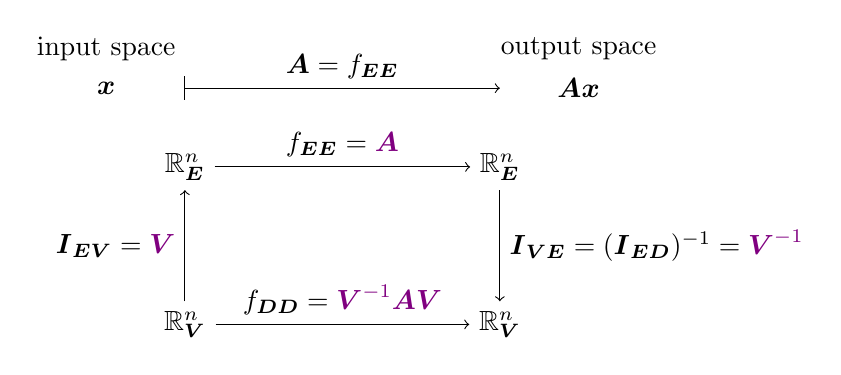
\begin{tikzpicture}
                        \node at (0, 0.5) {input space};
                        \node at (6, 0.5) {output space};

                        \node (x) at (0, 0) {$\vec{x}$};
                        \node (ax) at (6, 0) {$\mat{A}\vec{x}$};

                        \draw
                        (1, 0.15) -- (1, -0.15)
                        (1, 0) edge[->] node[above] {$\mat{A} = f_{\mat{E}\mat{E}}$} (5, 0);

                        \node (rel) at (1, -1) {$\mathbb{R}_{\mat{E}}^n$};
                        \node (rer) at (5, -1) {$\mathbb{R}_{\mat{E}}^n$};
                        \node (rvl) at (1, -3) {$\mathbb{R}_{\mat{V}}^n$};
                        \node (rvr) at (5, -3) {$\mathbb{R}_{\mat{V}}^n$};

                        \draw
                        (rvl) edge[->] node[left]{$\mat{I}_{\mat{E}\mat{V}} = \violet{\mat{V}}$} (rel)
                        (rel) edge[->] node[above]{$f_{\mat{E}\mat{E}} = \violet{\mat{A}}$} (rer)
                        (rer) edge[->] node[right] {$\mat{I}_{\mat{V}\mat{E}} = (\mat{I}_{\mat{E}\mat{D}})^{-1} = \violet{\mat{V}^{-1}}$} (rvr)
                        (rvl) edge[->] node[above]{$f_{\mat{D}\mat{D}} = \violet{\mat{V}^{-1}\mat{A}\mat{V}}$} (rvr);
                    \end{tikzpicture}
                \end{center}
                Consider a unit sphere, created by $|| \vec{x} || = 1$, where $\vec{x} \in \mathbb{R}^3$.
                The transformations $\mat{V}^{-1} = \mat{V}^\top$ and $\mat{V}$ are rotations as they preserve length.
                Take a point $\vec{x}$ on the surface of this unit sphere, applying $\mat{V}^{-1}$ to it simply rotates it to another point on the surface of the sphere (going from $\mathbb{R}_{\mat{E}}^3$ to $\mathbb{R}_{\mat{V}}^3$) in the input space.
                Let this point have coordinates $\vec{u}$ with respect to $\mat{V}$.
                Under the diagonal map $\text{diag}(\lambda_1, \dots, \lambda_n)$, we get the following;
                \begin{center}
                    $u_1 \vec{v_1} + \dots + u_n \vec{v_n} \mapsto \lambda_1 u_1 \vec{v_1} + \dots + \lambda_n u_n \vec{v_n}$
                \end{center}
                As $\vec{u}$ is on the sphere, we can say;
                \begin{center}
                    $|| \vec{u} ||_2^2 = u_1^1 + \dots + u_n^2 = 1$
                \end{center}
                Therefore, the mapped point $\vec{y}$ can be written as $\begin{bmatrix}
                    \lambda_1 u_1 \\ \vdots \\ \lambda_n u_n
                \end{bmatrix}$, satisfying (in three dimensions);
                $$\frac{y_1^2}{\lambda_1^2} + \frac{y_2^2}{\lambda_2^2} + \frac{y_3^2}{\lambda_3^2} = 1$$
                This gives a locus of an ellipsoid.
            \subsubsection*{Rank-Nullity Theorem}
                Take a matrix $\mat{A} \in \mathbb{R}^{m \times n}$.
                \begin{align*}
                    \text{Im}(\mat{A}) \subseteq \mathbb{R}^m & = \{ \mat{A}\vec{x} : \vec{x} \in \mathbb{R}^n\} \\
                    \text{dim}(\text{Im}(\mat{A})) & = \text{column rank of } \mat{A} \\
                    \text{Null}(\mat{A}) \subseteq \mathbb{R}^n & = \{ \vec{v} : \mat{A}\vec{v} = \vec{0} \} & \text{same as kernel} \\
                    \text{rk}(\text{column space}) & = \text{rk}(\text{row space}) \\
                    \text{row space } \mat{A} & = \text{column space } \mat{A}^\top
                \end{align*}
                For elementary row operations, we have the following property;
                \begin{enumerate}[(I)]
                    \itemsep0em
                    \item they are invertible.
                        \medskip

                        If there is one of the three elementary row operations $R$ that takes $\mat{A} \leadsto \mat{B}$, then $\exists R^{-1}$ that takes $\mat{B} \leadsto \mat{A}$.
                        \smallskip

                        If $\mat{A} \leadsto \mat{B}$, then $\mat{B} = \mat{M_R}\mat{A}$.
                        We obtain $\mat{M_R}$ by applying $R$ to $\mat{I}_m$, such that $\mat{I}_m \leadsto \mat{M_R}$.
                \end{enumerate}
                A reduction to row echelon form can be written as follows (with $-$ as a pivot, and $\times$ being any number);
                $$\mat{A} \overset{R_1}{\leadsto} \cdots \overset{R_t}{\leadsto} \mat{C} = \begin{bmatrix}
                    - & \times & \times & \times & \times & \times \\
                    0 & - & \times & \times & \times & \times \\
                    0 & 0 & 0 & - & \times & \times \\
                    0 & 0 & 0 & 0 & - & \times \\
                    0 & 0 & 0 & 0 & 0 & - \\
                    \hline
                    0 & 0 & 0 & 0 & 0 & 0
                \end{bmatrix}$$
                In general it creates a staircase of the pivots, and everything below it is 0.
                Note that the example above is just a random example, as long as the general structure remains, it's fine.
                \medskip

                An ERO doesn't change the row space, as it is operating on the rows.
                Swapping rows, multiplying by a non-zero number, and adding rows will not change anything.
                The claim is that while the column space can change, the rank of the column space doesn't change.
                \begin{align*}
                    \mat{A} & = [\vec{a_1}, \dots, \vec{a_n}] \\
                    \mat{A} \overset{R}{\leadsto} \mat{M_R}\mat{A} & = [\mat{M_R}\vec{a_1}, \dots, \mat{M_R}\vec{a_n}] \\
                    \mat{M_{R^{-1}}} & = (\mat{M_R})^{-1} & \text{therefore $\mat{M_R}$ is invertible}
                    \intertext{taking some linear combination of the vectors in $\mat{A}$}
                    \lambda_1 \vec{a_{i_1}} + \dots + \lambda_1 \vec{a_{i_t}} & = 0 & \Leftrightarrow \\
                    \mat{M_R}(\lambda_1 \vec{a_{i_1}} + \dots + \lambda_1 \vec{a_{i_t}}) & = 0
                \end{align*}
                This is due to the fact that multiplying a set of linearly independent vectors by an invertible matrix preserves independence.
                From this it follows that the dimension of the columns of $\mat{A}$ is equal to the dimension of the columns of $\mat{M_R}\mat{A}$, since $\mat{M_R}$ is invertible.
                Therefore neither the row rank nor the column rank changes.
                \medskip

                Since $\mat{C}$ is in REF, the row rank is equal to the column rank, which is equal to the number of pivots, let it be $r$, then $\text{rk}(\mat{A}) = r$.
\end{document}